\documentclass[ignorenonframetext,aspectratio=43]{beamer}
\setbeamertemplate{caption}[numbered]
\setbeamertemplate{caption label separator}{: }
\setbeamercolor{caption name}{fg=normal text.fg}
\beamertemplatenavigationsymbolsempty
\usepackage{lmodern}
\usepackage{amssymb,amsmath}
\usepackage{ifxetex,ifluatex}
\usepackage{fixltx2e} % provides \textsubscript
\ifnum 0\ifxetex 1\fi\ifluatex 1\fi=0 % if pdftex
  \usepackage[T1]{fontenc}
  \usepackage[utf8]{inputenc}
\else % if luatex or xelatex
  \ifxetex
    \usepackage{mathspec}
  \else
    \usepackage{fontspec}
  \fi
  \defaultfontfeatures{Ligatures=TeX,Scale=MatchLowercase}
\fi
\usecolortheme{beaver}
% use upquote if available, for straight quotes in verbatim environments
\IfFileExists{upquote.sty}{\usepackage{upquote}}{}
% use microtype if available
\IfFileExists{microtype.sty}{%
\usepackage{microtype}
\UseMicrotypeSet[protrusion]{basicmath} % disable protrusion for tt fonts
}{}
\newif\ifbibliography
\hypersetup{
            pdftitle={Recipes for multilevel imputation},
            pdfauthor={Stef van Buuren (Utrecht University)},
            pdfborder={0 0 0},
            breaklinks=true}
\urlstyle{same}  % don't use monospace font for urls
\usepackage{color}
\usepackage{fancyvrb}
\newcommand{\VerbBar}{|}
\newcommand{\VERB}{\Verb[commandchars=\\\{\}]}
\DefineVerbatimEnvironment{Highlighting}{Verbatim}{commandchars=\\\{\}}
% Add ',fontsize=\small' for more characters per line
\usepackage{framed}
\definecolor{shadecolor}{RGB}{248,248,248}
\newenvironment{Shaded}{\begin{snugshade}}{\end{snugshade}}
\newcommand{\KeywordTok}[1]{\textcolor[rgb]{0.13,0.29,0.53}{\textbf{#1}}}
\newcommand{\DataTypeTok}[1]{\textcolor[rgb]{0.13,0.29,0.53}{#1}}
\newcommand{\DecValTok}[1]{\textcolor[rgb]{0.00,0.00,0.81}{#1}}
\newcommand{\BaseNTok}[1]{\textcolor[rgb]{0.00,0.00,0.81}{#1}}
\newcommand{\FloatTok}[1]{\textcolor[rgb]{0.00,0.00,0.81}{#1}}
\newcommand{\ConstantTok}[1]{\textcolor[rgb]{0.00,0.00,0.00}{#1}}
\newcommand{\CharTok}[1]{\textcolor[rgb]{0.31,0.60,0.02}{#1}}
\newcommand{\SpecialCharTok}[1]{\textcolor[rgb]{0.00,0.00,0.00}{#1}}
\newcommand{\StringTok}[1]{\textcolor[rgb]{0.31,0.60,0.02}{#1}}
\newcommand{\VerbatimStringTok}[1]{\textcolor[rgb]{0.31,0.60,0.02}{#1}}
\newcommand{\SpecialStringTok}[1]{\textcolor[rgb]{0.31,0.60,0.02}{#1}}
\newcommand{\ImportTok}[1]{#1}
\newcommand{\CommentTok}[1]{\textcolor[rgb]{0.56,0.35,0.01}{\textit{#1}}}
\newcommand{\DocumentationTok}[1]{\textcolor[rgb]{0.56,0.35,0.01}{\textbf{\textit{#1}}}}
\newcommand{\AnnotationTok}[1]{\textcolor[rgb]{0.56,0.35,0.01}{\textbf{\textit{#1}}}}
\newcommand{\CommentVarTok}[1]{\textcolor[rgb]{0.56,0.35,0.01}{\textbf{\textit{#1}}}}
\newcommand{\OtherTok}[1]{\textcolor[rgb]{0.56,0.35,0.01}{#1}}
\newcommand{\FunctionTok}[1]{\textcolor[rgb]{0.00,0.00,0.00}{#1}}
\newcommand{\VariableTok}[1]{\textcolor[rgb]{0.00,0.00,0.00}{#1}}
\newcommand{\ControlFlowTok}[1]{\textcolor[rgb]{0.13,0.29,0.53}{\textbf{#1}}}
\newcommand{\OperatorTok}[1]{\textcolor[rgb]{0.81,0.36,0.00}{\textbf{#1}}}
\newcommand{\BuiltInTok}[1]{#1}
\newcommand{\ExtensionTok}[1]{#1}
\newcommand{\PreprocessorTok}[1]{\textcolor[rgb]{0.56,0.35,0.01}{\textit{#1}}}
\newcommand{\AttributeTok}[1]{\textcolor[rgb]{0.77,0.63,0.00}{#1}}
\newcommand{\RegionMarkerTok}[1]{#1}
\newcommand{\InformationTok}[1]{\textcolor[rgb]{0.56,0.35,0.01}{\textbf{\textit{#1}}}}
\newcommand{\WarningTok}[1]{\textcolor[rgb]{0.56,0.35,0.01}{\textbf{\textit{#1}}}}
\newcommand{\AlertTok}[1]{\textcolor[rgb]{0.94,0.16,0.16}{#1}}
\newcommand{\ErrorTok}[1]{\textcolor[rgb]{0.64,0.00,0.00}{\textbf{#1}}}
\newcommand{\NormalTok}[1]{#1}
\usepackage{longtable,booktabs}
\usepackage{caption}
% These lines are needed to make table captions work with longtable:
\makeatletter
\def\fnum@table{\tablename~\thetable}
\makeatother
\usepackage{graphicx,grffile}
\makeatletter
\def\maxwidth{\ifdim\Gin@nat@width>\linewidth\linewidth\else\Gin@nat@width\fi}
\def\maxheight{\ifdim\Gin@nat@height>\textheight0.8\textheight\else\Gin@nat@height\fi}
\makeatother
% Scale images if necessary, so that they will not overflow the page
% margins by default, and it is still possible to overwrite the defaults
% using explicit options in \includegraphics[width, height, ...]{}
\setkeys{Gin}{width=\maxwidth,height=\maxheight,keepaspectratio}

% Prevent slide breaks in the middle of a paragraph:
\widowpenalties 1 10000
\raggedbottom

\AtBeginPart{
  \let\insertpartnumber\relax
  \let\partname\relax
  \frame{\partpage}
}
\AtBeginSection{
  \ifbibliography
  \else
    \let\insertsectionnumber\relax
    \let\sectionname\relax
    \frame{\sectionpage}
  \fi
}
\AtBeginSubsection{
  \let\insertsubsectionnumber\relax
  \let\subsectionname\relax
  \frame{\subsectionpage}
}

\setlength{\parindent}{0pt}
\setlength{\parskip}{6pt plus 2pt minus 1pt}
\setlength{\emergencystretch}{3em}  % prevent overfull lines
\providecommand{\tightlist}{%
  \setlength{\itemsep}{0pt}\setlength{\parskip}{0pt}}
\setcounter{secnumdepth}{0}
\setbeamertemplate{footline}[text line]{%
  \parbox{\linewidth}{\vspace*{-8pt}Recipes for multilevel imputation - 190409 Utrecht\hfill\insertshortauthor\hfill\insertpagenumber}}
\setbeamertemplate{navigation symbols}{}

\title{Recipes for multilevel imputation}
\author{Stef van Buuren (Utrecht University)}
\date{April 9, 2019}

\begin{document}
\frame{\titlepage}

\begin{frame}{Main question}

\emph{Can we use MICE-algorithm for multilevel data, and if so, how?}

\end{frame}

\begin{frame}{Stochastic regression imputation}

\includegraphics{recipes_files/figure-beamer/unnamed-chunk-1-1.pdf}

\end{frame}

\begin{frame}{Missing data patterns, multivariate}

\includegraphics{recipes_files/figure-beamer/patterns-1.pdf}

\end{frame}

\begin{frame}{Three general strategies}

\begin{itemize}
\tightlist
\item
  Monotone data imputation
\item
  Joint modeling
\item
  Fully conditional specification (FCS)
\end{itemize}

\end{frame}

\begin{frame}{Imputation of monotone pattern}

\begin{center}\includegraphics{recipes_files/figure-beamer/unnamed-chunk-2-1} \end{center}

\end{frame}

\begin{frame}{Imputation of monotone pattern}

\begin{center}\includegraphics{recipes_files/figure-beamer/unnamed-chunk-3-1} \end{center}

\end{frame}

\begin{frame}{Imputation of monotone pattern}

\begin{center}\includegraphics{recipes_files/figure-beamer/unnamed-chunk-4-1} \end{center}

\end{frame}

\begin{frame}{Imputation of monotone pattern}

\begin{center}\includegraphics{recipes_files/figure-beamer/unnamed-chunk-5-1} \end{center}

\end{frame}

\begin{frame}{Imputation by joint modelling}

\begin{center}\includegraphics{recipes_files/figure-beamer/unnamed-chunk-6-1} \end{center}

\end{frame}

\begin{frame}{Imputation by joint modelling}

\begin{center}\includegraphics{recipes_files/figure-beamer/unnamed-chunk-7-1} \end{center}

\end{frame}

\begin{frame}{Imputation by joint modelling}

\begin{center}\includegraphics{recipes_files/figure-beamer/unnamed-chunk-8-1} \end{center}

\end{frame}

\begin{frame}{Imputation by joint modelling}

\begin{center}\includegraphics{recipes_files/figure-beamer/unnamed-chunk-9-1} \end{center}

\end{frame}

\begin{frame}{Imputation by joint modelling - next iteration}

\begin{center}\includegraphics{recipes_files/figure-beamer/unnamed-chunk-10-1} \end{center}

\end{frame}

\begin{frame}{Imputation by joint modelling - next iteration}

\begin{center}\includegraphics{recipes_files/figure-beamer/unnamed-chunk-11-1} \end{center}

\end{frame}

\begin{frame}{Imputation by fully conditional specification}

\begin{center}\includegraphics{recipes_files/figure-beamer/unnamed-chunk-12-1} \end{center}

\end{frame}

\begin{frame}{Imputation by fully conditional specification}

\begin{center}\includegraphics{recipes_files/figure-beamer/unnamed-chunk-13-1} \end{center}

\end{frame}

\begin{frame}{Imputation by fully conditional specification}

\begin{center}\includegraphics{recipes_files/figure-beamer/unnamed-chunk-14-1} \end{center}

\end{frame}

\begin{frame}{Imputation by fully conditional specification}

\begin{center}\includegraphics{recipes_files/figure-beamer/unnamed-chunk-15-1} \end{center}

\end{frame}

\begin{frame}{Imputation by fully conditional specification}

\begin{center}\includegraphics{recipes_files/figure-beamer/unnamed-chunk-16-1} \end{center}

\end{frame}

\begin{frame}{Imputation by fully conditional specification - next
iteration}

\begin{center}\includegraphics{recipes_files/figure-beamer/unnamed-chunk-17-1} \end{center}

\end{frame}

\begin{frame}{Imputation by fully conditional specification - next
iteration}

\begin{center}\includegraphics{recipes_files/figure-beamer/unnamed-chunk-18-1} \end{center}

\end{frame}

\begin{frame}{Which predictors?}

\begin{enumerate}
\def\labelenumi{\arabic{enumi}.}
\tightlist
\item
  Include all variables that appear in the complete-data model
\item
  Include variables related to the nonresponse
\item
  Include variables that explain a considerable amount of variance
\item
  Remove from variables selected in steps 2 and 3 those variables that
  have too many missing values within the subgroup of incomplete cases
\end{enumerate}

\emph{Does this recipe also apply to multilevel data?}

\end{frame}

\begin{frame}{\texttt{brandsma} data}

\begin{itemize}
\tightlist
\item
  Brandsma and Knuver, Int J Ed Res, 1989.
\item
  Extensively discussed in Snijders and Bosker (2012), 2nd ed.
\item
  4106 pupils, 216 schools, about 4\% missing values
\end{itemize}

\end{frame}

\begin{frame}[fragile]{\texttt{brandsma} data subset}

\begin{Shaded}
\begin{Highlighting}[]
\KeywordTok{library}\NormalTok{(mice)}
\NormalTok{d <-}\StringTok{ }\NormalTok{brandsma[, }\KeywordTok{c}\NormalTok{(}\StringTok{"sch"}\NormalTok{, }\StringTok{"lpo"}\NormalTok{, }\StringTok{"sex"}\NormalTok{, }\StringTok{"den"}\NormalTok{)]}
\KeywordTok{head}\NormalTok{(d, }\DecValTok{2}\NormalTok{)}
\end{Highlighting}
\end{Shaded}

\begin{verbatim}
##   sch lpo sex den
## 1   1  NA   1   1
## 2   1  50   1   1
\end{verbatim}

\begin{itemize}
\tightlist
\item
  \texttt{sch}: School number, cluster variable, \(C = 216\);
\item
  \texttt{lpo}: Language test post, outcome at pupil level;
\item
  \texttt{sex}: Sex of pupil, predictor at pupil level (0-1);
\item
  \texttt{den}: School denomination, predictor at school level (1-4).
\end{itemize}

\end{frame}

\begin{frame}[fragile]{Model of scientific interest}

Predict \texttt{lpo} from the

\begin{itemize}
\tightlist
\item
  level-1 predictor \texttt{sex}
\item
  level-2 predictor \texttt{den}
\end{itemize}

\end{frame}

\begin{frame}{Level notation - Bryk and Raudenbush (1992)}

\begin{align}
{{\texttt{lpo}}}_{ic} & = \beta_{0c} + \beta_{1c}{{\texttt{sex}}}_{ic} + \epsilon_{ic}\\
\beta_{0c}     & = \gamma_{00} + \gamma_{01}{{\texttt{den}}}_{c} + u_{0c}\\
\beta_{1c}     & = \gamma_{10}
\end{align}

\begin{itemize}
\tightlist
\item
  \(\text{lpo}_{ic}\) is the test score of pupil \(i\) in school \(c\)
\item
  \(\text{sex}_{ic}\) is the sex of pupil \(i\) in school \(c\)
\item
  \(\text{den}_c\) is the religious denomination of school \(c\)
\item
  \(\beta_{0c}\) is a random intercept that varies by cluster
\item
  \(\beta_{1c}\) is a sex effect, assumed to be the same across schools.
\item
  \(\epsilon_{ic} \sim N(0, \sigma_\epsilon^2)\) is the within-cluster
  random residual at the pupil level
\end{itemize}

\end{frame}

\begin{frame}{Where are the missings?}

In single level data, missingness may be in the outcome and/or in the
predictors

With multilevel data, missingness may be in:

\begin{enumerate}
\def\labelenumi{\arabic{enumi}.}
\item
  the outcome variable;
\item
  the level-1 predictors;
\item
  the level-2 predictors;
\item
  the class variable.
\end{enumerate}

\end{frame}

\begin{frame}{Univariate missing, level-1 outcome}

\begin{center}\includegraphics{recipes_files/figure-beamer/unnamed-chunk-20-1} \end{center}

\end{frame}

\begin{frame}{Univariate missing, level-1 predictor, sporadically
missing}

\begin{center}\includegraphics{recipes_files/figure-beamer/unnamed-chunk-21-1} \end{center}

\end{frame}

\begin{frame}{Univariate missing, level-1 predictor, systematically
missing}

\begin{center}\includegraphics{recipes_files/figure-beamer/unnamed-chunk-22-1} \end{center}

\end{frame}

\begin{frame}{Univariate missing, level-2 predictor}

\begin{center}\includegraphics{recipes_files/figure-beamer/unnamed-chunk-23-1} \end{center}

\end{frame}

\begin{frame}{Multivariate missing}

\begin{center}\includegraphics{recipes_files/figure-beamer/unnamed-chunk-24-1} \end{center}

\end{frame}

\begin{frame}{Nine challenges in multilevel imputation (1 of 3)}

\begin{enumerate}
\def\labelenumi{\arabic{enumi}.}
\item
  For small clusters the within-cluster mean and variance are unreliable
  estimates, so the choice of the prior distribution becomes critical.
\item
  For a small number of clusters, it is difficult to estimate the
  between-cluster variance of the random effects.
\item
  In applications with systematically missing data, there are no
  observed values in the cluster, so the cluster location cannot be
  estimated.
\end{enumerate}

\end{frame}

\begin{frame}{Nine challenges in multilevel imputation (2 of 3)}

\begin{enumerate}
\def\labelenumi{\arabic{enumi}.}
\setcounter{enumi}{3}
\item
  The variation of the random slopes can be large, and some methods have
  difficulty handling this.
\item
  The error variance \(\sigma_\epsilon^2\) may differ across clusters
  (heteroscedasticity), whereas the standard model assumes equal error
  variances.
\item
  The residual error distributions can be far from normal, e.g., for
  categorical data.
\end{enumerate}

\end{frame}

\begin{frame}{Nine challenges in multilevel imputation (3 of 3)}

\begin{enumerate}
\def\labelenumi{\arabic{enumi}.}
\setcounter{enumi}{6}
\item
  The model may contain aggregates of the level-1 variables, such as
  cluster means, which need to be taken in account during imputation.
\item
  The model may contain interactions, or other nonlinear terms.
\item
  It may not be possible to fit the multilevel model, or there are
  convergence problems.
\end{enumerate}

See \href{https://stefvanbuuren.name/fimd/sec-missmult.html}{Van Buuren
(2018)}

\end{frame}

\begin{frame}{Fully conditional specification}

\begin{align}
\dot{{\texttt{lpo}}}_{ic} & \sim N(\beta_0 + \beta_1 {{\texttt{den}}}_{c} + \beta_2 {{\texttt{sex}}}_{ic} + u_{0c}, \sigma_\epsilon^2)\\
\dot{{\texttt{sex}}}_{ic} & \sim N(\beta_0 + \beta_1 {{\texttt{den}}}_{c} + \beta_2 {{\texttt{lpo}}}_{ic} + u_{0c}, \sigma_\epsilon^2)
\end{align}

\end{frame}

\begin{frame}{Theoretical problem with FCS}

Conditional expectation of \(\texttt{sex}_{ic}\) in a random effects
model depends on

\begin{itemize}
\tightlist
\item
  \(\texttt{lpo}_{ic}\),
\item
  \(\overline{\texttt{lpo}}_{i}\), the mean of cluster \(i\), and
\item
  \(n_i\), the size of cluster \(i\).
\end{itemize}

Resche-Rigon \& White (2018) suggest the imputation model

\begin{itemize}
\tightlist
\item
  should incorporate the cluster means of level-1 predictors
\item
  be heteroscedastic if cluster sizes vary
\end{itemize}

\end{frame}

\begin{frame}{Univariate continuous multilevel imputation in
\texttt{mice}}

\begin{figure}
\centering
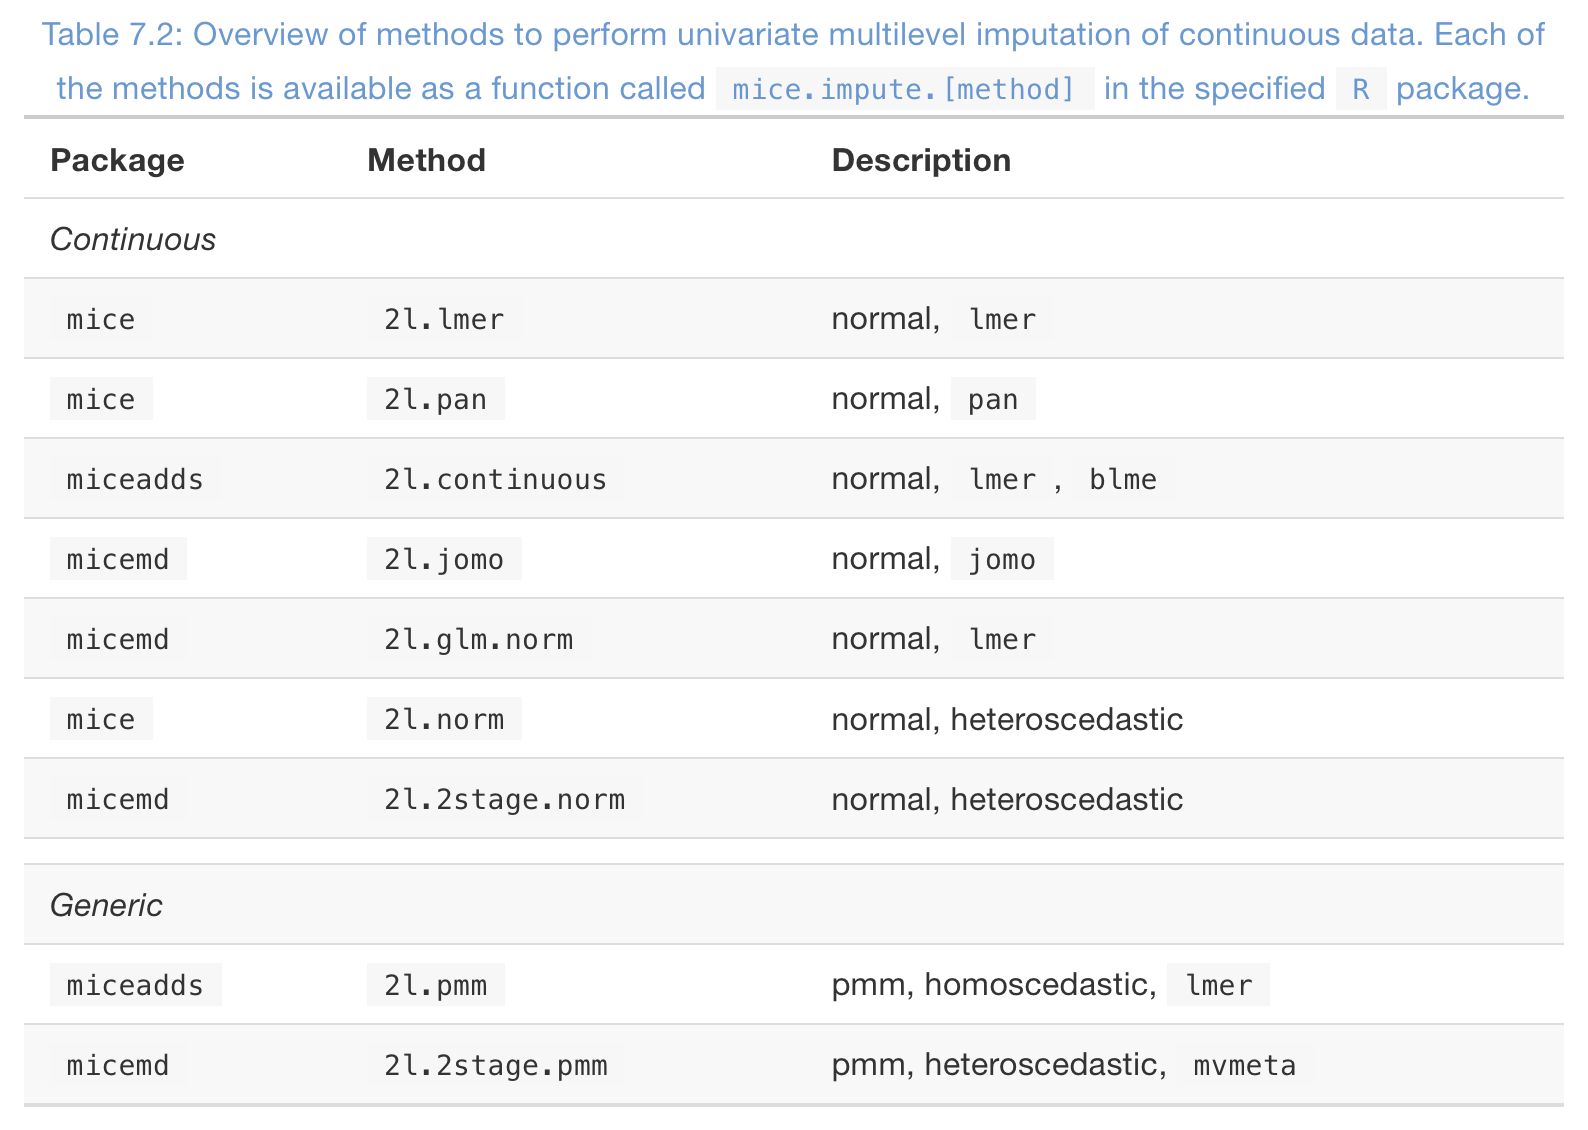
\includegraphics{figures/fig1.png}
\caption{}
\end{figure}

\end{frame}

\begin{frame}{Univariate binary and count multilevel imputation in
\texttt{mice}}

\begin{figure}
\centering
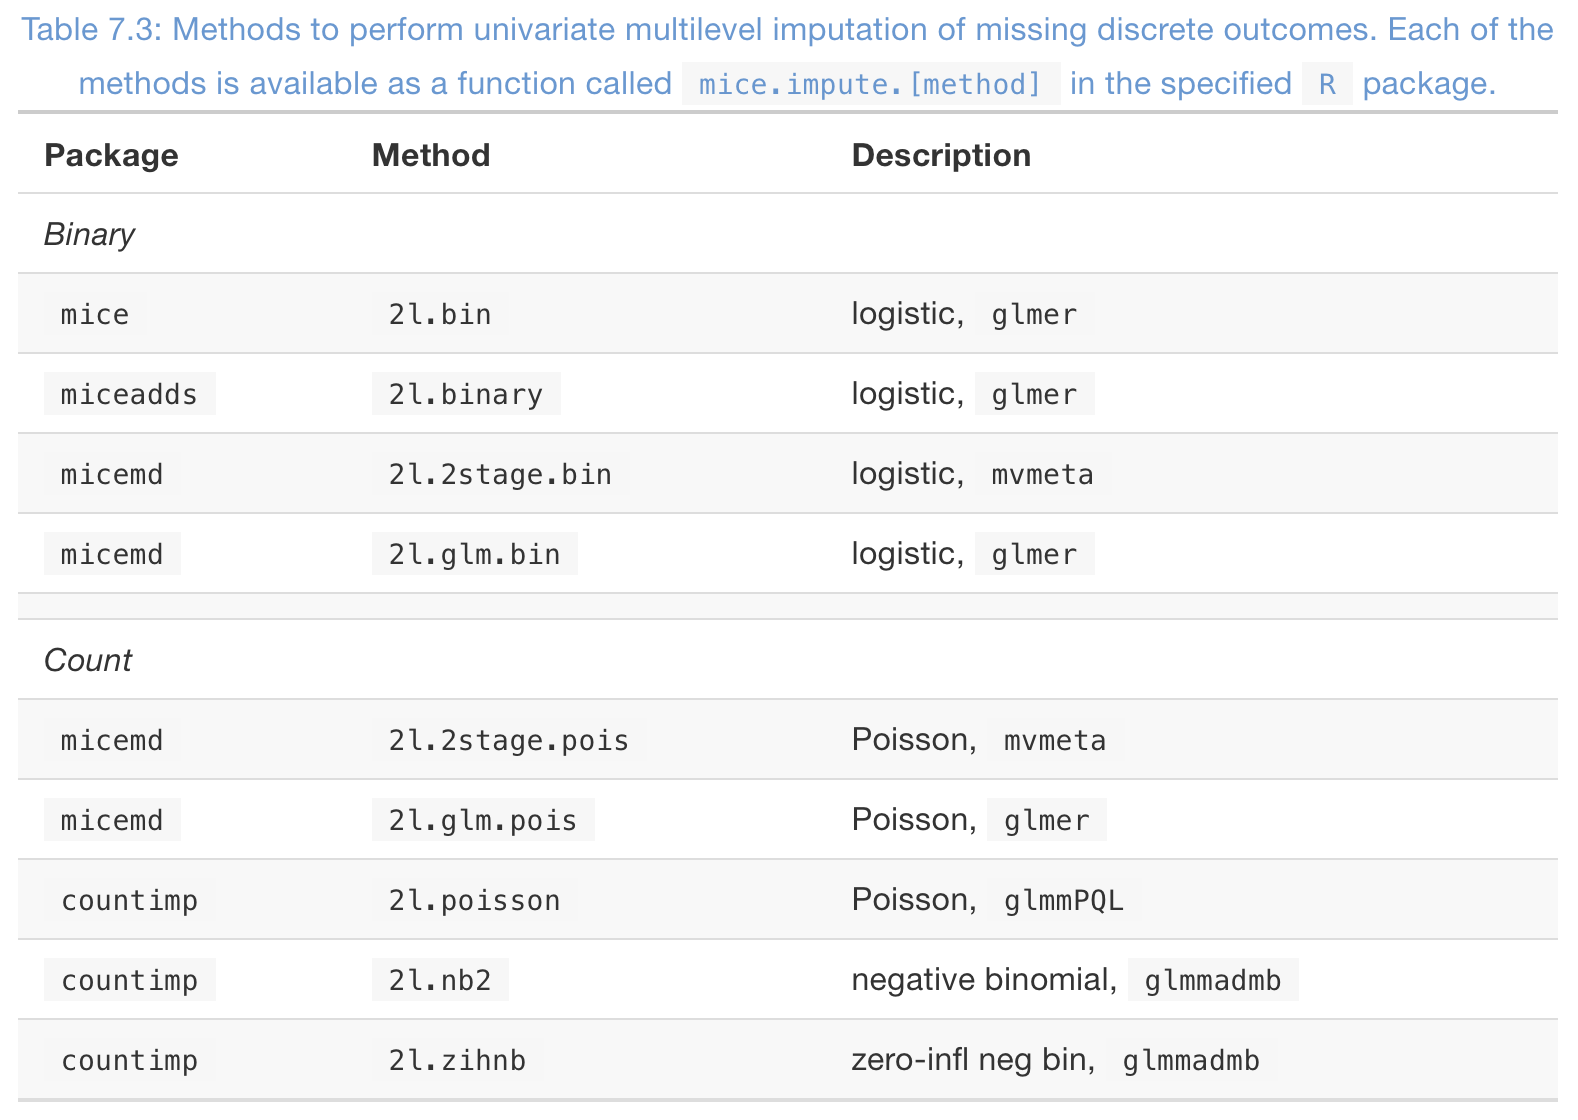
\includegraphics{figures/fig3.png}
\caption{}
\end{figure}

\end{frame}

\begin{frame}{Univariate level-2 imputation in \texttt{mice}}

\begin{figure}
\centering
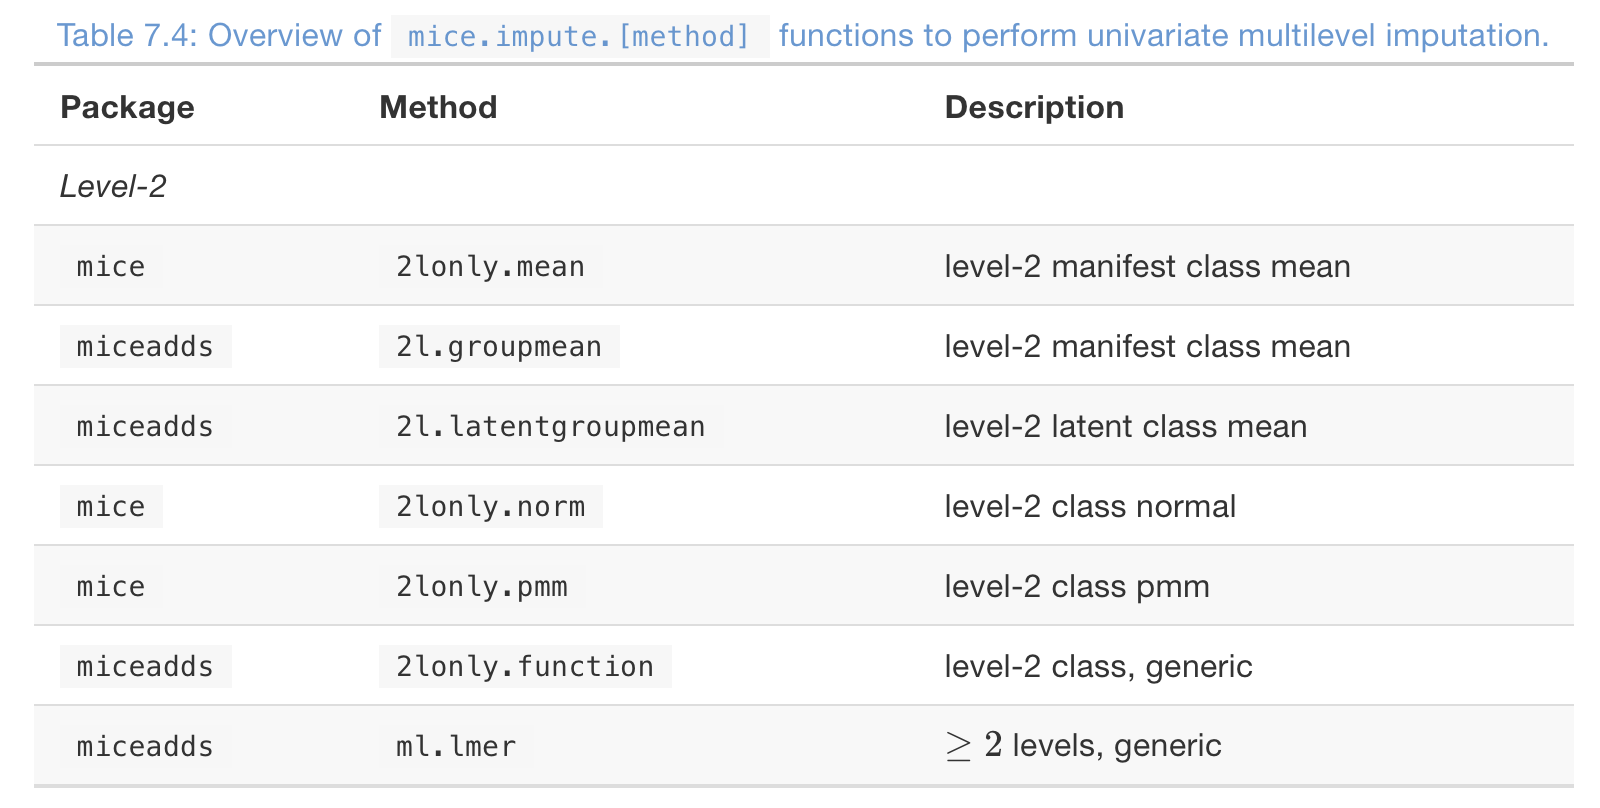
\includegraphics{figures/fig2.png}
\caption{}
\end{figure}

\end{frame}

\begin{frame}{General imputation/modeling sequence - START SIMPLE}

\begin{enumerate}
\def\labelenumi{\arabic{enumi}.}
\tightlist
\item
  Pick a simple complete-data model
\item
  Create imputations using an imputation template
\item
  Check the imputes (convergence/plausibility)
\item
  Estimate parameters
\item
  Make complete-data model more realistic, go to 1.
\end{enumerate}

See \url{https://stefvanbuuren.name/fimd/sec-mlguidelines.html}

\end{frame}

\begin{frame}{Seven imputation templates, increasing complexity}

\begin{enumerate}
\def\labelenumi{\arabic{enumi}.}
\tightlist
\item
  Intercept-only model, missing outcomes
\item
  Random intercepts, missing level-1 predictor
\item
  Random intercepts, contextual model
\item
  Random intercepts, missing level-2 predictor
\item
  Random intercepts, interactions
\item
  Random slopes, missing outcomes and predictors
\item
  Random slopes, interactions
\end{enumerate}

\end{frame}

\begin{frame}{1 Intercept-only model, missing outcomes (model)}

\begin{align}
{{\texttt{lpo}}}_{ic} & = \beta_{0c} + \epsilon_{ic}\\
\beta_{0c}     & = \gamma_{00} + u_{0c}
\end{align}

\end{frame}

\begin{frame}[fragile]{1 Intercept-only model, missing outcomes
(imputation)}

\begin{Shaded}
\begin{Highlighting}[]
\NormalTok{d <-}\StringTok{ }\NormalTok{brandsma[, }\KeywordTok{c}\NormalTok{(}\StringTok{"sch"}\NormalTok{, }\StringTok{"lpo"}\NormalTok{)]}
\NormalTok{pred <-}\StringTok{ }\KeywordTok{make.predictorMatrix}\NormalTok{(d)}
\NormalTok{pred[}\StringTok{"lpo"}\NormalTok{, }\StringTok{"sch"}\NormalTok{] <-}\StringTok{ }\OperatorTok{-}\DecValTok{2}
\NormalTok{imp <-}\StringTok{ }\KeywordTok{mice}\NormalTok{(d, }\DataTypeTok{pred =}\NormalTok{ pred, }\DataTypeTok{meth =} \StringTok{"2l.pmm"}\NormalTok{, }\DataTypeTok{m =} \DecValTok{10}\NormalTok{, }\DataTypeTok{maxit =} \DecValTok{1}\NormalTok{,}
            \DataTypeTok{print =} \OtherTok{FALSE}\NormalTok{, }\DataTypeTok{seed =} \DecValTok{152}\NormalTok{)}
\end{Highlighting}
\end{Shaded}

\end{frame}

\begin{frame}[fragile]{1 Intercept-only model, missing outcomes
(analysis)}

\begin{Shaded}
\begin{Highlighting}[]
\KeywordTok{library}\NormalTok{(lme4)}
\end{Highlighting}
\end{Shaded}

\begin{verbatim}
## Loading required package: Matrix
\end{verbatim}

\begin{Shaded}
\begin{Highlighting}[]
\NormalTok{fit <-}\StringTok{ }\KeywordTok{with}\NormalTok{(imp, }\KeywordTok{lmer}\NormalTok{(lpo }\OperatorTok{~}\StringTok{ }\NormalTok{(}\DecValTok{1} \OperatorTok{|}\StringTok{ }\NormalTok{sch), }\DataTypeTok{REML =} \OtherTok{FALSE}\NormalTok{))}
\KeywordTok{summary}\NormalTok{(}\KeywordTok{pool}\NormalTok{(fit))}
\end{Highlighting}
\end{Shaded}

\begin{verbatim}
##             estimate std.error statistic   df p.value
## (Intercept)     40.9     0.322       127 3368       0
\end{verbatim}

\end{frame}

\begin{frame}[fragile]{1 Intercept-only model, missing outcomes
(variances)}

\begin{Shaded}
\begin{Highlighting}[]
\KeywordTok{library}\NormalTok{(mitml)}
\KeywordTok{testEstimates}\NormalTok{(}\KeywordTok{as.mitml.result}\NormalTok{(fit), }\DataTypeTok{var.comp =} \OtherTok{TRUE}\NormalTok{)}\OperatorTok{$}\NormalTok{var.comp}
\end{Highlighting}
\end{Shaded}

\begin{verbatim}
##                          Estimate
## Intercept~~Intercept|sch   18.021
## Residual~~Residual         63.306
## ICC|sch                     0.222
\end{verbatim}

\end{frame}

\begin{frame}[fragile]{2 Random intercepts, missing level-1 (model)}

\begin{align}
{{\texttt{lpo}}}_{ic} & = \beta_{0c} + \beta_{1c}{{\texttt{iqv}}}_{ic} + \epsilon_{ic}\\
\beta_{0c}     & = \gamma_{00} + u_{0c}\\
\beta_{1c}     & = \gamma_{10}
\end{align}

\begin{itemize}
\tightlist
\item
  Missing values in both \texttt{lpo} and \texttt{iqv}
\end{itemize}

\end{frame}

\begin{frame}[fragile]{2 Random intercepts, missing level-1
(imputation)}

\begin{Shaded}
\begin{Highlighting}[]
\NormalTok{d <-}\StringTok{ }\NormalTok{brandsma[, }\KeywordTok{c}\NormalTok{(}\StringTok{"sch"}\NormalTok{, }\StringTok{"lpo"}\NormalTok{, }\StringTok{"iqv"}\NormalTok{)]}
\NormalTok{pred <-}\StringTok{ }\KeywordTok{make.predictorMatrix}\NormalTok{(d)}
\NormalTok{pred[}\StringTok{"lpo"}\NormalTok{, ] <-}\StringTok{ }\KeywordTok{c}\NormalTok{(}\OperatorTok{-}\DecValTok{2}\NormalTok{, }\DecValTok{0}\NormalTok{, }\DecValTok{3}\NormalTok{)}
\NormalTok{pred[}\StringTok{"iqv"}\NormalTok{, ] <-}\StringTok{ }\KeywordTok{c}\NormalTok{(}\OperatorTok{-}\DecValTok{2}\NormalTok{, }\DecValTok{3}\NormalTok{, }\DecValTok{0}\NormalTok{)}
\NormalTok{imp <-}\StringTok{ }\KeywordTok{mice}\NormalTok{(d, }\DataTypeTok{pred =}\NormalTok{ pred, }\DataTypeTok{meth =} \StringTok{"2l.pmm"}\NormalTok{, }\DataTypeTok{seed =} \DecValTok{919}\NormalTok{,}
            \DataTypeTok{m =} \DecValTok{10}\NormalTok{, }\DataTypeTok{print =} \OtherTok{FALSE}\NormalTok{)}
\end{Highlighting}
\end{Shaded}

\begin{itemize}
\tightlist
\item
  Impute \texttt{lpo} from \texttt{iqv} \emph{and} the cluster means of
  \texttt{iqv}
\item
  Impute \texttt{iqv} from \texttt{lpo} \emph{and} the cluster means of
  \texttt{lpo}
\item
  Alternative: Use \texttt{mitml::panImpute()} or
  \texttt{mitml::jomoImpute()}
\end{itemize}

\end{frame}

\begin{frame}[fragile]{2 Random intercepts, missing level-1
(predictorMatrix)}

\begin{Shaded}
\begin{Highlighting}[]
\NormalTok{pred}
\end{Highlighting}
\end{Shaded}

\begin{verbatim}
##     sch lpo iqv
## sch   0   1   1
## lpo  -2   0   3
## iqv  -2   3   0
\end{verbatim}

\end{frame}

\begin{frame}[fragile]{2 Random intercepts, missing level-1 (analysis)}

\begin{Shaded}
\begin{Highlighting}[]
\NormalTok{fit <-}\StringTok{ }\KeywordTok{with}\NormalTok{(imp, }\KeywordTok{lmer}\NormalTok{(lpo }\OperatorTok{~}\StringTok{  }\NormalTok{iqv }\OperatorTok{+}\StringTok{ }\NormalTok{(}\DecValTok{1} \OperatorTok{|}\StringTok{ }\NormalTok{sch), }\DataTypeTok{REML =} \OtherTok{FALSE}\NormalTok{))}
\KeywordTok{summary}\NormalTok{(}\KeywordTok{pool}\NormalTok{(fit))}
\end{Highlighting}
\end{Shaded}

\begin{verbatim}
##             estimate std.error statistic   df p.value
## (Intercept)    40.96    0.2378       172 3337       0
## iqv             2.52    0.0525        48 2127       0
\end{verbatim}

\begin{Shaded}
\begin{Highlighting}[]
\KeywordTok{testEstimates}\NormalTok{(}\KeywordTok{as.mitml.result}\NormalTok{(fit), }\DataTypeTok{var.comp =} \OtherTok{TRUE}\NormalTok{)}\OperatorTok{$}\NormalTok{var.comp}
\end{Highlighting}
\end{Shaded}

\begin{verbatim}
##                          Estimate
## Intercept~~Intercept|sch    9.479
## Residual~~Residual         40.862
## ICC|sch                     0.188
\end{verbatim}

\end{frame}

\begin{frame}[fragile]{4 Random intercepts, missing level-2 predictor
(model)}

\begin{align}
{{\texttt{lpo}}}_{ic} & = \beta_{0c} + \beta_{1c}{{\texttt{iqv}}}_{ic} + \epsilon_{ic}\\
\beta_{0c}     & = \gamma_{00} + \gamma_{01}{{\texttt{den}}}_{c} + u_{0c}\\
\beta_{1c}     & = \gamma_{10}
\end{align}

\begin{itemize}
\tightlist
\item
  Missing values in \texttt{lpo}, \texttt{iqv} and \texttt{den}
\item
  For \texttt{den} the imputation model uses school level aggregates
\end{itemize}

\end{frame}

\begin{frame}[fragile]{4 Random intercepts, missing level-2
(imputation)}

\begin{Shaded}
\begin{Highlighting}[]
\NormalTok{d <-}\StringTok{ }\NormalTok{brandsma[, }\KeywordTok{c}\NormalTok{(}\StringTok{"sch"}\NormalTok{, }\StringTok{"lpo"}\NormalTok{, }\StringTok{"iqv"}\NormalTok{, }\StringTok{"den"}\NormalTok{)]}
\NormalTok{meth <-}\StringTok{ }\KeywordTok{make.method}\NormalTok{(d)}
\NormalTok{meth[}\KeywordTok{c}\NormalTok{(}\StringTok{"lpo"}\NormalTok{, }\StringTok{"iqv"}\NormalTok{, }\StringTok{"den"}\NormalTok{)] <-}\StringTok{ }\KeywordTok{c}\NormalTok{(}\StringTok{"2l.pmm"}\NormalTok{, }\StringTok{"2l.pmm"}\NormalTok{,}
                                  \StringTok{"2lonly.pmm"}\NormalTok{)}
\NormalTok{pred <-}\StringTok{ }\KeywordTok{make.predictorMatrix}\NormalTok{(d)}
\NormalTok{pred[}\StringTok{"lpo"}\NormalTok{, ] <-}\StringTok{ }\KeywordTok{c}\NormalTok{(}\OperatorTok{-}\DecValTok{2}\NormalTok{, }\DecValTok{0}\NormalTok{, }\DecValTok{3}\NormalTok{, }\DecValTok{1}\NormalTok{)}
\NormalTok{pred[}\StringTok{"iqv"}\NormalTok{, ] <-}\StringTok{ }\KeywordTok{c}\NormalTok{(}\OperatorTok{-}\DecValTok{2}\NormalTok{, }\DecValTok{3}\NormalTok{, }\DecValTok{0}\NormalTok{, }\DecValTok{1}\NormalTok{)}
\NormalTok{pred[}\StringTok{"den"}\NormalTok{, ] <-}\StringTok{ }\KeywordTok{c}\NormalTok{(}\OperatorTok{-}\DecValTok{2}\NormalTok{, }\DecValTok{1}\NormalTok{, }\DecValTok{1}\NormalTok{, }\DecValTok{0}\NormalTok{)}
\NormalTok{imp <-}\StringTok{ }\KeywordTok{mice}\NormalTok{(d, }\DataTypeTok{pred =}\NormalTok{ pred, }\DataTypeTok{meth =}\NormalTok{ meth, }\DataTypeTok{seed =} \DecValTok{418}\NormalTok{,}
            \DataTypeTok{m =} \DecValTok{10}\NormalTok{, }\DataTypeTok{print =} \OtherTok{FALSE}\NormalTok{)}
\end{Highlighting}
\end{Shaded}

\end{frame}

\begin{frame}[fragile]{4 Random intercepts, missing level-2
(predictorMatrix)}

\begin{Shaded}
\begin{Highlighting}[]
\NormalTok{pred}
\end{Highlighting}
\end{Shaded}

\begin{verbatim}
##     sch lpo iqv den
## sch   0   1   1   1
## lpo  -2   0   3   1
## iqv  -2   3   0   1
## den  -2   1   1   0
\end{verbatim}

\end{frame}

\begin{frame}{4 Random intercepts, missing level-2 (density)}

\includegraphics{recipes_files/figure-beamer/mladenspmm-1.pdf}

\end{frame}

\begin{frame}[fragile]{4 Random intercepts, missing level-2 (analysis)}

\begin{verbatim}
##                 estimate std.error statistic   df  p.value
## (Intercept)       40.071    0.4549     88.09  187 0.000000
## iqv                2.516    0.0532     47.34 1242 0.000000
## as.factor(den)2    2.041    0.5925      3.45  430 0.000626
## as.factor(den)3    0.234    0.6519      0.36  285 0.719431
## as.factor(den)4    1.843    1.1642      1.58 1041 0.113755
\end{verbatim}

\begin{verbatim}
##                          Estimate
## Intercept~~Intercept|sch    8.621
## Residual~~Residual         40.761
## ICC|sch                     0.175
\end{verbatim}

\end{frame}

\begin{frame}[fragile]{Recipe: Missing level-1}

\begin{longtable}[]{@{}ll@{}}
\toprule
& Recipe for a level-1 target\tabularnewline
\midrule
\endhead
1. & Define the most general analytic model\tabularnewline
2. & Select a \texttt{2l} method that imputes close to the
data\tabularnewline
3. & Include all level-1 variables\tabularnewline
4. & Include the disaggregated cluster means of level-1
variables\tabularnewline
5. & Include all level-1 interactions implied by analytic
model\tabularnewline
6. & Include all level-2 predictors\tabularnewline
7. & Include all level-2 interactions implied by analytic
model\tabularnewline
8. & Include all cross-level interactions implied by analytic
model\tabularnewline
9. & Include predictors related to the missingness and the
target\tabularnewline
10. & Exclude any terms involving the target\tabularnewline
\bottomrule
\end{longtable}

\end{frame}

\begin{frame}[fragile]{Recipe: Missing level-2}

\begin{longtable}[]{@{}ll@{}}
\toprule
& Recipe for a level-2 target\tabularnewline
\midrule
\endhead
1. & Define the most general analytic model\tabularnewline
2. & Select a \texttt{2lonly} method that imputes close to the
data\tabularnewline
3. & Include the cluster means of all level-1 variables\tabularnewline
4. & Include the cluster means of all level-1
interactions\tabularnewline
5. & Include all level-2 predictors\tabularnewline
6. & Include all interactions of level-2 variables\tabularnewline
7. & Include predictors related to the missingness and
target\tabularnewline
8. & Exclude any terms involving the target\tabularnewline
\bottomrule
\end{longtable}

\end{frame}

\begin{frame}{Conclusion}

\emph{Can we use MICE-algorithm for multilevel data, and if so, how?}

\begin{itemize}
\tightlist
\item
  Hot spot of current research
\item
  Multilevel imputation: more complex, but doable
\item
  Start simple, take small steps
\item
  Build upon templates and modeling recipes
\item
  Study \url{https://stefvanbuuren.name/fimd/sec-mlguidelines.html}
\item
  Gain confidence at each step
\item
  Start playing around\ldots{}
\end{itemize}

\end{frame}

\end{document}
